\section{Introduction}
\label{sec:introduction}
\subsection{Background}
Open cooling systems must deliver relief despite continuous exchange with their surroundings. Fans alter human convective and evaporative losses; evaporative coolers also change air temperature and moisture \cite{fanguide,evapequip}. Comparing them requires useful service per unit energy.

\subsection{Problem Restatement}
The five tasks are to define cooling efficiency, develop bus and rail models, test two contrasting venues, extend efficiency into an effectiveness decision, and communicate operating guidance through a memorandum and public blog \cite{problem}.

\subsection{Our Modeling Framework}
Our \textbf{CP-SET Framework (Coupled Psychrometric-SET Service Efficiency \& Effectiveness Framework)} connects conserved heat and moisture to local exposure, then converts SET relief into person-time service per kWh. Requirements 1--3 compare efficiency; Requirement 4 adds cooling adequacy, visitor experience and cost. The workflow below preserves this progression.
\begin{center}
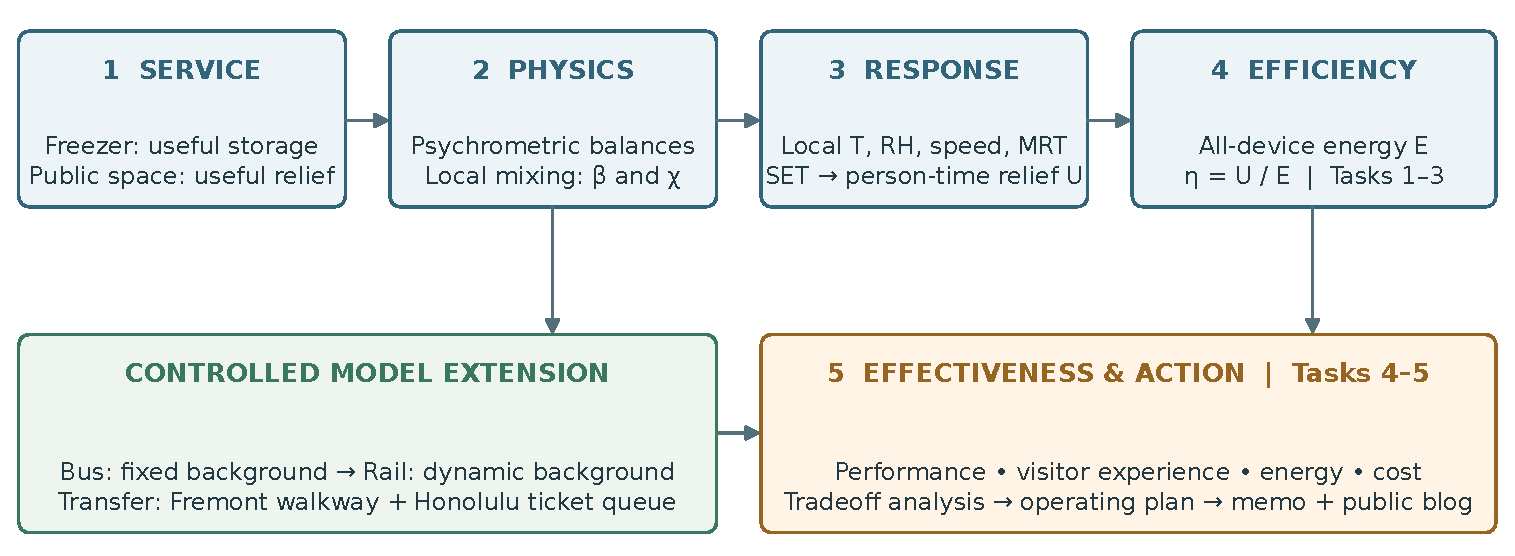
\includegraphics[width=\linewidth]{figures/29_cp_set_framework.pdf}\\[-2pt]
{\small\textbf{CP-SET workflow.} A shared physical and service model supports progressively broader decisions.}
\end{center}
\ifinlineai
\noindent\footnotesize AI assistance in model development, coding and writing is documented in the appended report \cite{codex,gemini}.\normalsize
\fi
